
%3. Study of variance between models and data.  The optimized models part of this section is predicated on result 1b (so that optimization results can be believed).  You already have the poster for this.
%I think this captures most of your results in three themes.  Other results which are really methods, like parallel rheobase search, can stay in the methods, and you will get credit for them there.

\section{Published models vs optimized models}
\label{sec:optimizing-published-models}
It is known that neural models and experimental measurements generally diverge in important ways, however, it is desirable to know the specific sources of divergence. Models and experiments may disagree for two reasons: \emph{A} the model is not flexible enough to satisfy a particular constraint simultaneously to a collection of constraints, or, \emph{B} the model was incorrectly fitted to the a type of conflicting constraints (for example model fitted to spike times at the expense of Rheobase, and FISlope). 

Since we don't yet have complete knowledge of model/experiment divergence, we don't necessarily know the best features to target with regards to model fitting. Specific knowledge of model/data disagreement facilitates the prioritized selection of features that should guide optimization. 

%\begin{figure}
%    \centering
%    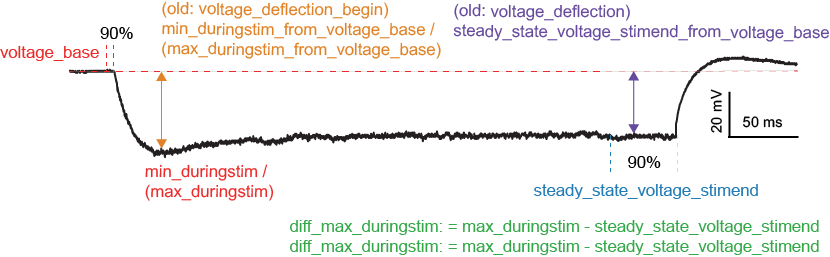
\includegraphics{figures/voltage_features.png}
%    \caption{Caption}
%    \label{fig:voltage_figures}
%\end{figure}
%\begin{figure}
%    \centering
%    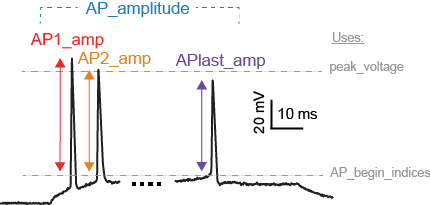
\includegraphics{figures/AP_Amplitude.png}
%    \caption{Caption}
%    \label{fig:features_example}
%\end{figure}

%\begin{figure}
%    \centering
%    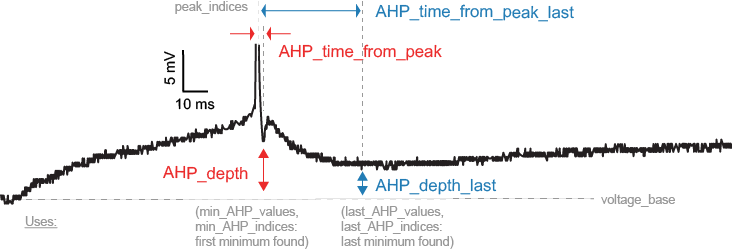
\includegraphics{figures/AHP.png}
%    \caption{After hyperpolarisation potential }
%    \label{fig:features_example_ahp}
%\end{figure}


%\begin{figure}
%    \centering
%    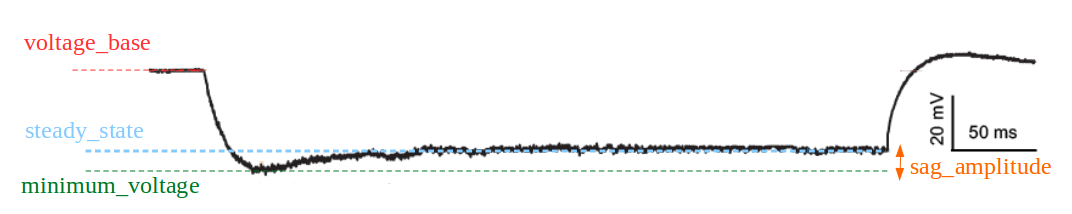
\includegraphics{figures/sag_amplitude}
%    \caption{Caption}
%    \label{fig:sag_amplitude}
%\end{figure}


\subsection{Features} 

For many of these features it will be useful to refer back to the methods \ref{sec:data_sources} section, where I some key features were depicted. 

Consider a voltage recording at the location of the membrane of a neuron. Teams of researchers have already segmented voltage recordings into labelled sections, each section has a classification that is based on the shape of waveform in a limited region see figure \ref{fig:voltage_figures} for example. Rather than specifying by name each measurement it is often useful to refer collectively to these measurable shapes as "features". 

In the following multivariate analysis we analyze hundreds of such features, and we summarize important differences in a subset of this high dimensional feature space.  Below, I describe some neuronal model features that agreed well with experiments, and some features that diverged.


\subsection{Publications Associated with Model Sources}
$972$ models, $448$ experiments.
$1276$ samples. This did not include some blue brain cells. After data cleaning many data points were dropped.  $244$
$1420$


Allen Institute for Brain Science Cell Types Database \citep{celltypes} can be accessed using the SDK.
The Blue Brain Project Dataset \citep{toledo} can be obtained from the Data Navigator, or an API.

\begin{itemize}
\item Allen Institute V1 \cite{gouwens2018systematic}
\item Somatosensory Cortex \cite{markram2006blue} 
\end{itemize}

\subsubsection{Feature Extraction Libraries}
\begin{table}
\centering
%\resizebox{\textwidth}{!}{
\begin{tabular}{lll}
%\toprule
{} EFEL Ephys Feature Extraction Library & AllenSDK & Druckmann (2012) 
%\bottomrule
\end{tabular}
%}
\end{table}




%\begin{tabular}{lll}
%\toprule
%{} Injection 1 & Injection 2 & %Injection 3 \\
% at $1.0 \times$ Rheobase & at $1.5 %\times$ Rheobase & at $3.0 \times$ %Rheobase 
%\bottomrule
%\end{tabular}




%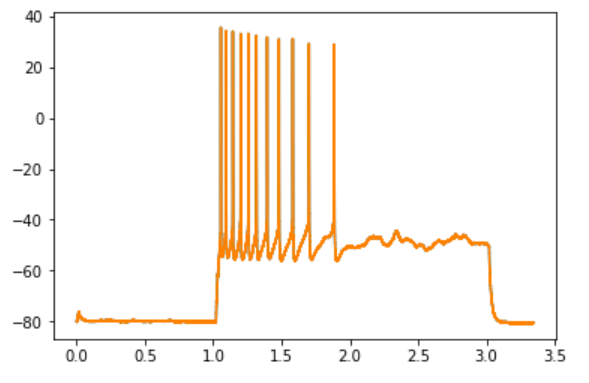
\includegraphics[]{chapters/app_tex/Allen_rush}
\begin{figure}
    \begin{center}
    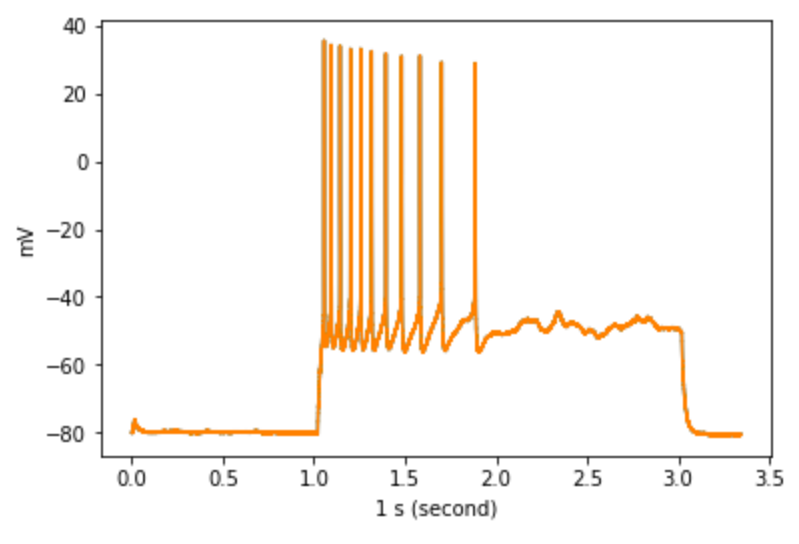
\includegraphics[width=0.6\linewidth]{figures/multi_spiking_large_allen}
    \caption{A voltage recording from a supra-threshold experiment waveform used as a basis for the Allen Brain Institute cell types data base. Publication Gouwens rat \citep{gouwens2018systematic}}
    \label{fig:adaptionm}
    \end{center}
\end{figure}    

\begin{figure}  
    \begin{center}
    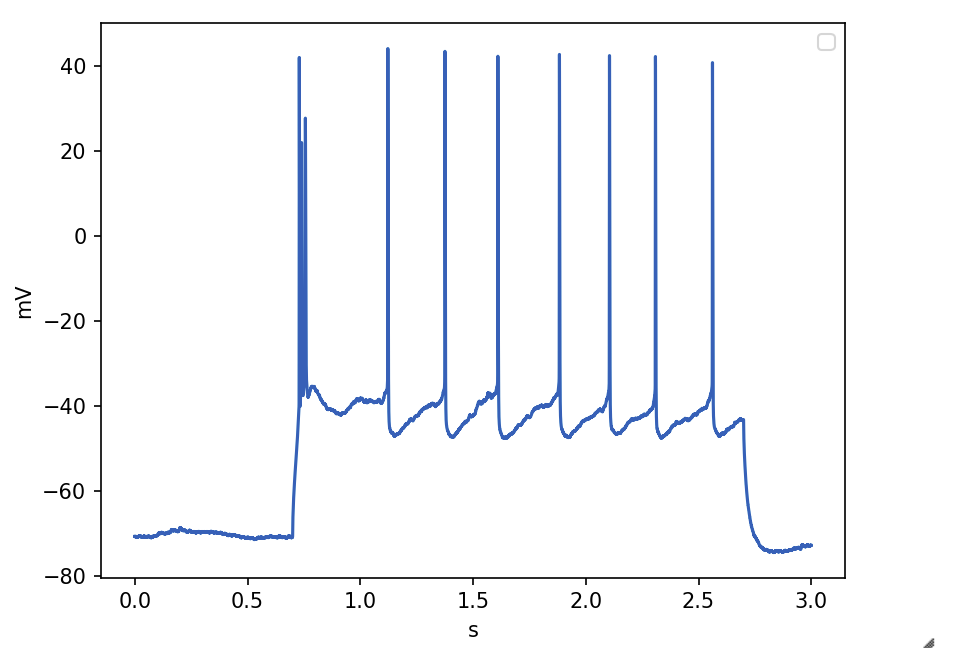
\includegraphics[width=0.6\linewidth]{figures/multi_spiking_large_bbp}
    \caption{Another example of a supra threshold experimental protocol. Publication Jouvanile rat \citep{toledo}}
    \label{fig:bbp_trace_adaption_late_spike}
    \end{center}
\end{figure}    

In order to identify electrical measurements or "features" that were responsible for the most variance in models and in-vitro, we performed Sparse Principle Component Analysis \citep{zou2006sparse} on the combined pool of model and \emph{in vitro} experiments. 

\subsection{Sources of Model/Experiment Disagreement}
The key advantage of using sparse PCA is the results are readily interpret able. 
A common sceanario in regular Principal Component Analysis is you may obtain a low dimensional embedding plot made from unit rotation vectors that maximize variance, but no way of relating the reduced dimensions back to the sources of variance in the system of interest. 

Sparse PCA yields an interpretable list of features, that build the principle components.
This list of features is ranked and sorted with respect to their total contributions to the Eigen Vectors. Since two Eigen Vectors where made these are.

Principle component 1 had non zero loadings for ranked (highest to lowest).
The first Eigen Vector does not facilitate discrimination between models and experiments, but the second Eigen Vector spaces models and experiments into three seperate clusters.

\begin{table}
\begin{tabular}{lll}
\toprule
{} Injection 1 & Injection 2 & Injection 3 \\
 at $1.0 \times$ Rheobase & at $1.5 \times$ Rheobase & at $3.0 \times$ Rheobase 

\end{tabular}
\caption[Model Specific, Three Step Stimulus Protocol]{Under the three step protocol rheobase current is determined uniquely for each model or experiment. Then mutiples of rheobase are applied for two increasingly stronger rheobase strengths at $\times 1.5$ and $\times 3.0 Rheobase$.
In experiments these protocols had already been run, but a re-organising of those preexisting experiments was required in order to make the experiments consistent with the model evaluation scheme.}
\end{table}

Principle component 2 had non zero loadings for ranked (highest to lowest)
\begin{table}
\resizebox{\textwidth}{!}{
\begin{tabular}{llll}
\toprule

Feature Name & Feature Description & Extraction Library &  Stimulus Strength \\
 upstroke-t & The time of upstrokes, this is the below $V_{T}$ first upward phase of AP & Allen & $1.5 \times$ Rheobase\\
 peak-t & Time(s) maximum $V_{M}$ occurs & Allen & $1.5 \times$ Rheobase \\
threshold-t & Time(s) $V_{T}$ is surpassed & Allen & $1.5 \times$ Rheobase \\
fast-trough-t & Description & Allen & $1.5 \times$ Rheobase \\ 
fast-trough-t & Same as above but at $3 \times$ Rheobase & Allen & $3.0 \times$ Rheobase \\
upstroke-t & Same as above but at $3 \times$ Rheobase & Allen & $3.0 \times$ Rheobase \\ 
peak-t & Same as above but at $3 \times$ Rheobase &Allen & $3.0 \times$ Rheobase \\ 
threshold-t & Same as above but at $3 \times$ Rheobase & Allen & $3.0 \times$ Rheobase \\ 
peak-indices & Indexs into array where peak voltages occur & EFEL & $1.5 \times$ Rheobase \\
min-AHP-indices & Indexs into array where minimum After Hyperpolarisation occur & EFEL & $1.5 \times$ Rheobase \\
\bottomrule
\end{tabular}
}
\caption[Features of first principal component in sparse PCA]{Features of first principal component in sparse PCA. It is notable that Principle component one described variance, common to both models and experiments, it did not seperate models and experiments into different clusters.}

\end{table}

\begin{table}
\resizebox{\textwidth}{!}{
\begin{tabular}{llll}
\toprule
Feature Name & Feature Description & Extraction Library  & Stimulus Strength \\
fast-trough-index & Description & Allen & $1.5 \times$ Rheobase\\
peak-index-1.5x & Description & Allen & $1.5 \times$ Rheobase \\
upstroke-index-1.5x & Description & Allen & $1.5 \times$ Rheobase \\
threshold-index-1.5x & Description & Allen & $1.5 \times$ Rheobase \\ 
fast-trough-time & Description & Allen & $1.5 \times$ Rheobase \\
fast-trough-index-3.0x & Description & Allen & $3.0 \times$ Rheobase \\ 
peak-index-3.0x & Description & Allen & $3.0 \times$ Rheobase \\
upstroke-index-3.0x & Description & Allen & $3.0 \times$ Rheobase \\ 
threshold-index-3.0x & Description & Allen & $3.0 \times$ Rheobase \\
\bottomrule
\end{tabular}}
\caption[Features of second principal component in sparse PCA]{Features of second principal component in sparse PCA. It is notable that mainly these features contributed to the seperation of model and experiment clusters}
\end{table}

Adaptation index 1 and adaptation 2 are the same but adaptation 2 evaluates for when there are skipped peaks. A skipped peak is when a spike or a spiklet does not surpass the nominated threshold for spike detection. 

%The parameter \myid{spike skipf} is the fraction of skipped peaks, $k$ is the minimum of \myid{spike skipf} times $N$ and \myid{max spike skip}.

% FAIL "Minimum 4 spike needed for feature [adaptation\_index]." \- \\
The adaptation index is defined as "the Normalized average difference of two consecutive ISIs". "The adaptation index is zero for a constant firing rate and bigger than zero for a decreasing firing rate \citep{EFEL}"

  %All peaks in the time interval of \myid{stim start}$-$\myid{offset} and \myid{stim end}$+$\myid{offset} are regarded, \myid{offset} defaults to zero.
  
%pt$_0, \ldots, $pt$_{n-1} =$ peak\_time \\
%  pt$'_0$, \ldots, pt$'_{m-1}$  = $\{$ pt$_i$ | pt$_i \ge$ stim\_start $-$ offset AND pt$_i \le$ stim\_end $+$ offset $\}$ \\
%  $k = \min \{$ spike\_skipf $\cdot m$, max\_spike\_skip$\}$ \\
%  pt$''_0$, \ldots, pt$''_{l-1}$ = (pt$'_k$, \ldots, pt$'_m$) \\
%  IF $l$ < 4 THEN \+ \\
%    FAIL "Minimum 4 spike needed for feature [adaptation\_index]." \- \\
%  ENDIF \\
%  isi$_0$, \ldots, isi$_{j-1} =$ pt$''_1 -$ pt$''_0$, \ldots, pt$''_{l-1} -$ pt$''_{l-2}$ \\
%  sub$_0$, \ldots, sub$_{i-1} =$ isi$_1 -$ isi$_0$, \ldots, isi$_{j-1} -$ isi$_{j-2}$ \\
%  sum$_0$, \ldots, sum$_{i-1} =$ isi$_1 +$ isi$_0$, \ldots, isi$_{j-1} +$ isi$_{j-2}$ \\
%  APPEND $\frac{1}{i-1} \sum_{n=0}^{i-1} \frac{\mathrm{sub}_n}{\mathrm{sum}_n}$ TO adaptation\_index}
 % All peaks in the time interval of \myid{stim start}$-$\myid{offset} and \myid{stim end}$+$\myid{offset} are regarded, \myid{offset} defaults to zero.
The adaptation index is zero for a constant firing rate and bigger than zero for a decreasing firing rate:
  


%Adaptation index 2  {Normalized average difference of two consecutive ISIs}

% The parameter \myid{spike skipf} is the fraction of skipped peaks, $k$ is the minimum of \myid{spike skipf} times $N$ and \myid{max spike skip}.

\url{https://github.com/BlueBrain/eFEL/blob/master/docs/source/tex/efeatures.tex#L382}

These are the weighted features that were used to make Eigen vectors 1 and 2, are responsible for most of the variance. Interestingly these features mostly belong to the Allen SDK feature extraction set, with two exceptions: $peak-indices-1.5x$ $min-AHP-indices-1.5 \times$ belonging to EFEL efel 

%Move to Discussion 
Another observation is that a small majority of features used to create the sparse Eigen Vectors, are in the range of $1.5 \times$  rheobase, and slightly fewer are features from a $3.0\times$ rheobase experiment. A reason for this is as follows, larger spike time variability $C_{V}$ is expressed in intermediate ranges of current injection. Under the highest current injections, high frequency evenly spaced spikes are likely, although spike frequency adaption is possible, the higher current may force to spikes to occur promptly after their refractory period, and in this case you might observe diminishing amplitude of spikes with increasing stimulus duration.

At $1.5 \times rheobase $ I believe there to be more spike time variation, at $3.0 \times rheobase $  I believe there to be more spike amplitude variation.

\subsection{Sparse PCA}


%The first principle component 
Models and experiments shared the same breadth of variability across the first principal component, with only slightly more variance in the experiments than in the data. Allen cell types experiments seemed to encompass the most variability out of models and experiments across all data sets see the right figure inset in \ref{fig:pca_data_points}. Models clustered tightly and varied less than in vitro experiments. There was one group of Allen cell type experiments that clustered on their own, making one set of the cluster.


Although imputation was successfully used to avoid dropping a large number of samples, about half of all initial BBP/Allen models data types were excluded from a final analysis, because they did not all capable of meeting inclusion criteria.  

\ref{fig:reference_feature_list}
List of complete 47 features used in the analysis down from 466 after data cleaning.

Sparse PCA 2nd Eigen Vector. 
Disagreement between models and in-vivo neurons may reflect limitations of model design and can be investigated by probing the key features used by classifiers to distinguish these two populations. 

\begin{figure}    
\begin{center} 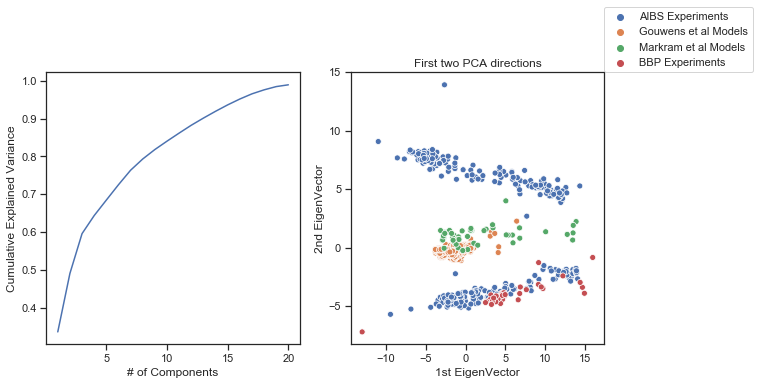
\includegraphics[width=1.0\linewidth]{figures/cortical_model_data_agreement_52_1}
    \caption[Is this visible]{}
    \label{fig:}
\end{center}
\caption[Sparse PCA, variance explained, 1st and 2nd Principal Components]{Sparse PCA revealed five overlapping different groups of neuronal identity's, and three non overlapping clusters. Models and experiments clustered separately to each other in the low dimensional space. Models and data were easily separable in the direction of the 2nd Eigen Vector.}
\label{fig:pca_data_points}
\end{figure}    



\begin{figure}    
    \begin{center}
    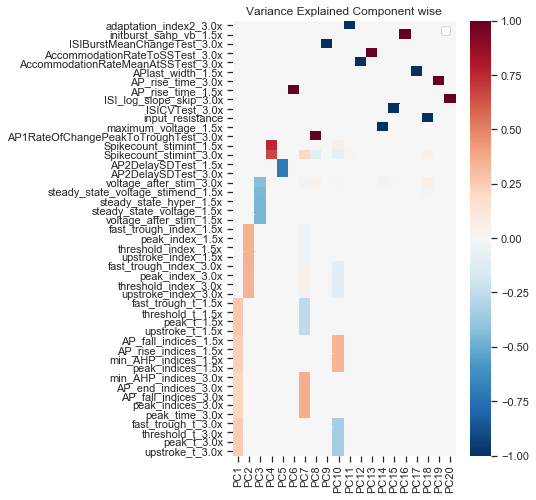
\includegraphics[scale=0.75]{figures/cortical_model_data_agreement_54_1.png}
    \caption[Component Loadings used to make Eigen Vectors of sparse PCA]{}
    
    
    
%fast_trough_indexes : numpy array of indexes at the start of the trough (i.e. end of the spike)
%adp_indexes : numpy array of adp indexes (np.nan if there was no ADP in that ISI
%slow_trough_indexes : numpy array of indexes at the minimum of the slow phase of the trough
    \end{center}
\end{figure}    
\cite{wang2019sag}

\begin{figure}
    \centering
    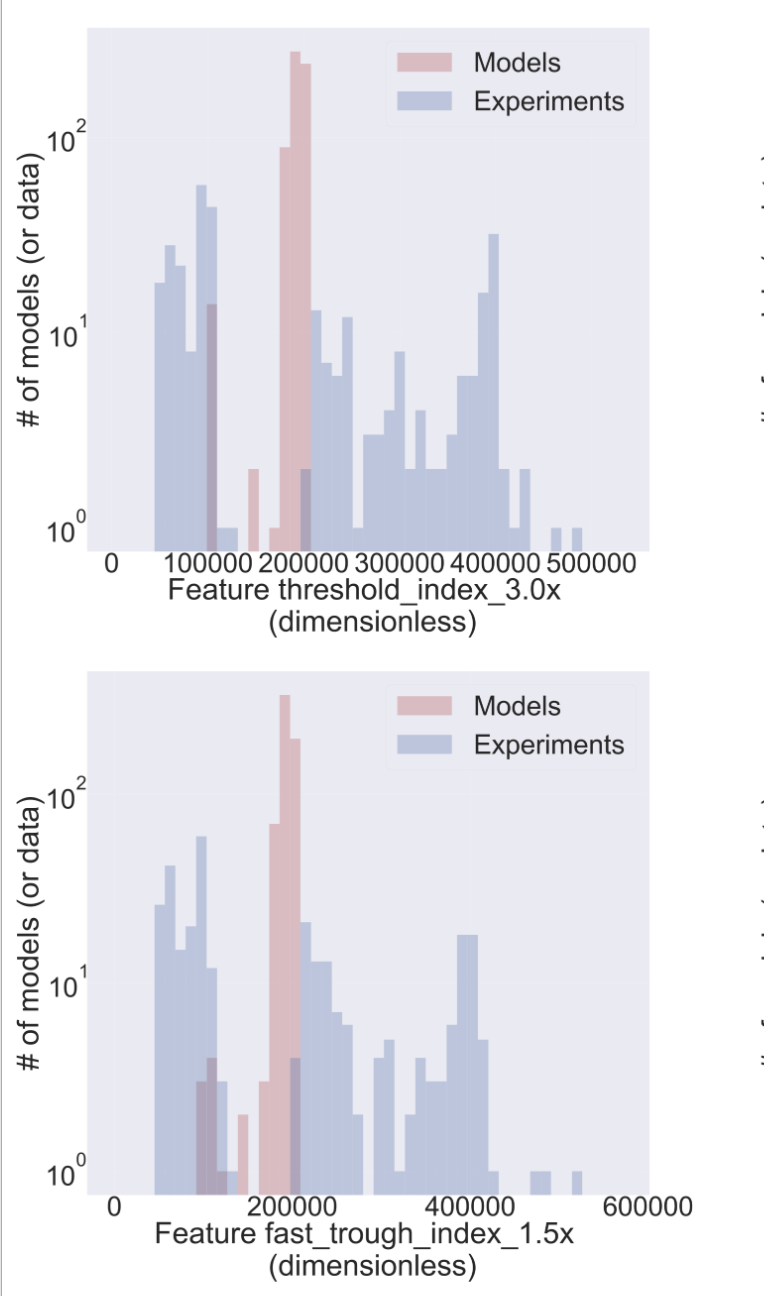
\includegraphics[scale=0.75]{figures/features_that_disagree}
    \caption[Features that disagree. Slow Trough indexs, from the Allen cell types feature extraction]{The sparse PCA graph is very abstract, it's important to understand that much variance found by the sparse PCA algorithm originates from differences between model distributions and experiment distributions Simple stacked histograms of data are able to show such differences. By "Fast" in fast trough indexs, all that is meant is the beginning time of troughs occurrence, this would contrast with the "slow" or ending time of the spikes. This is arguably a bad naming scheme.
    \url{https://allensdk.readthedocs.io/en/latest/allensdk.ephys.ephys_features.html}
    }
        \label{fig:from_poster_disagree}
\end{figure}



\begin{comment}
\begin{itemize}
    \item upstroke\_t\_1.5x allen feature
    \item  peak\_t\_1.5x allen feature
    \item threshold\_t\_1.5x allen feature
    \item fast\_trough\_t\_1.5x allen feature
    \item fast\_trough\_t\_3.0x allen feature
    \item upstroke\_t\_3.0x allen feature
    \item peak\_t\_3.0x allen feature
    \item threshold\_t\_3.0x allen feature
    \item peak\_indices\_1.5x efel feature
    \item min\_AHP\_indices\_1.5x efel feature
\end{itemize}
\end{comment}


%\begin{itemize}
%    \item fast\_trough\_index\_1.5x allen feature
%    \item fast\_trough\_index\_3.0x allen feature
%    \item threshold\_index\_1.5x allen feature
%    \item peak\_index\_1.5x allen feature
%    \item upstroke\_index\_1.5x allen feature
%    \item peak\_index\_3.0x allen feature
%    \item upstroke\_index\_3.0x allen feature
%    \item threshold\_index\_3.0x allen feature
%\end{itemize}

After identifying specific sources of model and experiment divergence, it is now possible in theory to start fitting models which seek to resolve specific types of disagreement.
However, as alluded to in the introduction, it was found that were two other important factors. 

%Model repurposing is common and it is done on a network scale \cite{traub} and an individual cell scale.
%Experimental evidence is starting to reveal that model re-purposing of pyramidal neurons might not be a good idea.

%Scientific insight is well-served by the discovery and optimization of abstract models that can reproduce experimental findings. NeuroML (NeuroML.org), a model description language for neuroscience, facilitates reproducibility and exchange of such models by providing an implementation-agnostic model description in a modular format. NeuronUnit (neuronunit.scidash.org) evaluates model accuracy by subjecting models to experimental data-driven validation tests, a formalization of the scientific method. 


% After applying dimensionality reduction to this very high dimensional feature space, we show that the real (biological neurons) and simulated (model neurons) recordings are easiley and fully discriminated by eye or any reasonable classifier.  

% Are they still discernable?
%972 models, 448 experiments.


%Consequently, not a single model neuron produced physiological responses that could be confused with a biological neuron. Was this a defect of the model design (e.g. key mechanisms unaccounted for) or of model parameterization? We found that if we introduced models that were revised via optimization the revised models overlapped with the distribution of biological neurons, and were mostly classified as such. 
